\documentclass[a4paper]{article}
\title{L8}
\author{Hanwen Jin}
\usepackage[utf8]{inputenc}
\usepackage[T1]{fontenc}
\usepackage{amsmath, amssymb}
\usepackage{tikz}
\usepackage{amsthm}
\usepackage{graphicx}
\usepackage{float}
% figure support
\usepackage{import}
\usepackage{transparent}
\newcommand{\incfig}[1]{%
	\def\svgwidth{\columnwidth}
	\import{./figures/}{#1.pdf_tex}
}
\theoremstyle{definition}
\newtheorem{definition}{Definition}[section]
\newtheorem{example}{Example}[section]
\newtheorem{theorem}{Theorm}[section]
\newtheorem{corollary}{Corollary}[theorem]
\newtheorem{lemma}[theorem]{Lemma}
\newtheorem{exercise}{Exercise}[section]
\newtheorem*{remark}{Remark}
\pdfsuppresswarningpagegroup=1

\begin{document}
	\maketitle
	Conservation law
	\begin{equation}
		\begin{cases}
			u_t+uu_x=0,t\in \left( 0,\infty \right) ,x\in \mathbb{R}\\
			u\left( 0,x \right) =f\left( x \right) ,x\in \mathbb{R}
		\end{cases}
	\end{equation} 	
	Characteristic system: $x-tf\left( \tau \right) =\tau$, $\frac{d}{dt}\left( u\left( t,x-tf\left( \tau \right)  \right)  \right) =0$

	$u\left( t,x-tf\left( \tau \right)  \right) =f\left( \tau \right) $. 
	Can we invert $x-tf\left( \tau \right) =\tau$? If we can then $\implies \tau =f\left( x,t \right) $

	Implicit function theorem : Assume $F\in C^{1}\left( \mathbb{R}^{3} \right) $, $F=F\left( t,x,\tau \right) =0$ , suppose at some point $\left( t_0,x_0,\tau_0 \right) $ , we know that $\frac{\partial F}{\partial \tau} \not =0$, $\implies \exists g, $ such that $\tau=g\left( x,t \right) , g\in C^{1}$. In a neighbourhood of $t_0,x_0$. 

	Inversion is possible in the union of all neighbourhood of point where above is statified. 

	In our case, $F\left( t,x,\tau \right) =x-tf\left( \tau \right) =\tau$. Inversion set= $\left\{ \left( x,t,\tau \right): \frac{\partial F}{\partial \tau} \not = 0  \right\} $. 
	\begin{equation}
		\frac{\partial F }{\partial \tau} \not = 0 \iff 1+tf'\left( \tau \right) \not = 0
	\end{equation} 
	Assume $f\in C^{1}$, $\left|f'\left( x \right) \le M  \right|\forall x $ for some $M>0$. if $t<\frac{1}{M}$, then $1+t\left( f'\left( \tau \right)  \right) \ge 1-t\left|f'\left( \tau \right)  \right|\ge 1-Mt \ge 0$. 

	This is loval existance theorem: if $f\in C^{1} \left( \mathbb{R} \right) :\left|f'\left( x \right)  \right| \le M \forall x\in \mathbb{R}$, then there exist unique classical solution of Burger's equation. 

	If $f'\left( \tau \right) \ge 0$, $\forall \tau\implies_1+tf'\left( \tau\ge 1>0 \right) \forall t>0$, the condition of classical solution always fullfill, solution is global in time. In this case, 
	\begin{theorem}[]
		If $f\in C^{1}\left( \mathbb{R} \right) $, then the solution to Burger equation is global iff f is non decreasing. We have proved $\impliedby$ , what about $\implies?$. 

		If $f $ decreases, then there are $\tau_1,\tau_2$ such that $f\left( \tau_1 \right) <f\left( \tau_2 \right) $. Follow characteristics. 

		$x-tf\left( \tau_1 \right) =\tau_1$, $u$ is constant and = $f\left( \tau_1 \right) $ .. . (1)

		$x-tf\left( \tau_2 \right) =\tau_2$, $u$ is constant and $=f\left( \tau_2 \right) $ .. . (2) 

		We will hsow that they intercept. so $u=f\left( \tau_1  \right)  $ and $u=f\left( \tau_2  \right)$, so u is not continuous. 

		(2)-(1): $t\left( f\left( \tau_1 \right) -f\left( \tau_2 \right)  \right) =\tau_2-\tau_1$
		\begin{equation}
			t=\frac{\tau_2-\tau_1}{f\left( \tau_1 \right) -f\left( \tau_2 \right) }\implies \text{characteristic intercepts}
		\end{equation} 
		at this t, which is positive, $\implies $ solution become discontinuous, hencen ot global. 
	\end{theorem}
	\paragraph{Graphical interpreteationo}%
	Case 1: if $f'\left( \tau \right) \ge 0 \forall \tau$ then f is increasing. $t=\frac{1}{f\left( \tau \right) }x-\frac{\tau}{f\left( \tau \right) }$. 
	Then we have 
	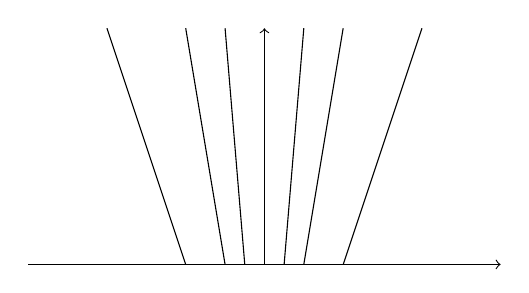
\begin{tikzpicture}
	\draw[->](-3,0)--(3,0);
	\draw[->](0,0)--(0,3);
	\draw[](0.25,0)--(0.5,3);
	\draw[](-0.25,0)--(-0.5,3);
	\draw[](0.5,0)--(1,3);
	\draw[](-0.5,0)--(-1,3);
	\draw[](-1,0)--(-2,3);
	\draw[](1,0)--(2,3);
	\end{tikzpicture}
	
	Case 2: $f'\left( \tau  \right) <0$ , $f $ is decreasing. 
	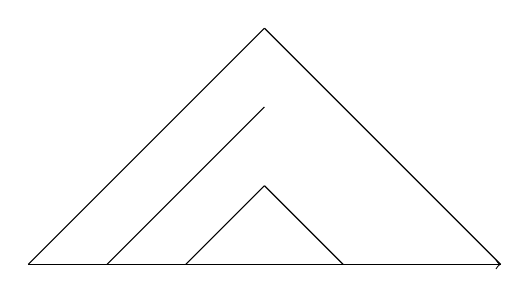
\begin{tikzpicture}
	\draw[->](-3,0)--(3,0);
	\draw[](0,0)--(3,0);
	\draw[](-1,0)--(0,1);
	\draw[](1,0)--(0,1);
	\draw[](-2,0)--(0,2);
	\draw[](-3,0)--(0,3);
	\draw[](3,0)--(0,3);
	\end{tikzpicture}
	There are points of discontinuity. 

	What happens to solution in case 2? We have local solution up to $t<\frac{1}{M}$, for f decreasing, $f'\left( \tau \right) \le M$. $Q:t\to \frac{1}{M}$? let $\tau_*$ be such that $f'\left( \tau _*\right) =-M $. 

	$x-f\left( \tau_* \right) =\tau_*$, 
	\begin{align*}
		\label{eq:jdkf}
		u\left( t,x  \right) =f\left( \tau \right) f\left( x-tf\left( \tau \right)  \right) \\
		u\left( t,x  \right) =f\left( x-tu \left( t,x  \right)  \right) \\
		u_x &= f'\left( x-tu \right) \cdot \left( 1-tu_x \right)  \\&\implies u_x=\frac{f'\left( x-tu \right) }{1+tf'\left( x-tu \right) }
	\end{align*}
	Take $t\to \frac{1}{M }$ on the characteristic, $x-tf\left( \tau \right) =\tau_*$. 
	\begin{equation}
	\frac{f'\left( x-tu \right) }{1+tf'\left( x-tu \right) }\to \frac{-M }{1-tM} \to \infty \text{as $t\to \frac{1}{M}$}	\end{equation} 
	u stops being C. 
	
\end{document}
